\documentclass[aspectratio=169]{beamer}
%% For 4:3 aspect ratio:
%% \documentclass{beamer}
\usepackage{../git-course}

\title[git-course]{An Introduction to \gh\ and \gs}
\author{Chris Grandin \& Andrew Edwards}
\date{\today}

\begin{document}
%% Needed to remove 'Figure:' from figure captions:
\setbeamertemplate{caption}{\raggedright\insertcaption\par}

\frame[plain]{
\titlepage
}

\section{Introduction}

\section{Creating/Cloning}
\frame{\frametitle{Creating a new repository}
  \bi
    \item Sign into your \gh\ account, click on the
      \emph{Repositories} tab, and press the \emph{New} button.
    \item Give your repository a name. Let's call it \lstinline{test}.
    \item Check \emph{Initialize this repository with a README}.
    \item Leave \emph{Add .gitignore} and \emph{Add a license}
      set to \emph{None}.
    \item Click \emph{Create repository}.
  \ei
}

\frame{\frametitle{Cloning your new repository}
  \bi
    \item Once you have created the \lstinline{test} repository on \gh, copy
      the URL of the repository.
    \item Open the \gs\ and run the following command to clone your repository:
      \lstinline{git clone URL test}\\
      where \lstinline{URL} is the url of your newly created repository. You
      can paste the \lstinline{URL} into the command line (on Windows) by
      pressing the right mouse button.
  \ei
  \bigskip
  You should now have a subdirectory called \lstinline{test}. In \gs, change
  to that directory:\\
  \lstinline{cd test}
}

\frame{\frametitle{Windows only: Storing your credentials}
  When you are using the \gs\ for the first time, issue
  the following command:\\
  \bigskip
  \lstinline{git config --global credential.helper wincred}\\
  \bigskip
  This means that you don't have to repeatedly enter your \gh\ password.\\
  The command creates a credential file containing your account information:\\
  \lstinline[escapechar="\\"]{C:\\Users\\YOUR-COMPUTER-USER-NAME\\.git-credentials}\\
}

\section{Committing new files}
\begingroup
\small
\frame{\frametitle{Copy and commit \emph{.gitignore}}
  \bi
    \item Copy the \emph{.gitignore} file from the git-course directory and
      paste it into your newly cloned directory. You can edit this to suit
      the project, as there is a different \emph{.gitignore} file for each
      project.
    \item Check the status of your repository: \lstinline{git status}
    \item You will see that the new file \emph{.gitignore} has not been
      staged for commit. It is an \emph{Untracked file}. You need to add any
      new files to be committed by using the \lstinline{git add} command:\\
      \lstinline{git add .gitignore}
    \item Make a commit for the changes:\\
      \lstinline{git com "Added .gitignore"}\\
      The commit message should be a useful message saying what the commit
      encapsulates.\\
      Note the git command \lstinline{com} is an alias for the more complex
      command: \lstinline{git commit -a -m "Added .gitignore"}\\
      Aliases are found in your \lstinline{.gitconfig} file. You can make
      up your own as you see fit.
    \item Push the commit to \gh: \lstinline{git push}
    \item Check the \gh\ webpage and see your commit and that the file
      has been uploaded.
  \ei
}
\endgroup

\frame{\frametitle{Edit \emph{Readme.md}}
  Edit the \emph{Readme.md} file. Add some simple comments describing
  the project such as: "A test repository for learning Git."\\
  \bigskip
  Look over the changes, commit them, and push them to your \gh\
  repository:\\
  \lstinline{git s}\\
  \lstinline{git diff}\\
  \lst{git com "Initial edit of Readme.md"}\\
  \lst{git push}\\
  ~\\
  Refresh your \gh\ web page and you should see your text 
  (the \emph{Readme.md} file is what is shown on the main page
  of your repo).
}

\frame{\frametitle{Copy, edit and commit \emph{simpleText.txt}}
  \bn
    \item Copy the text file \lst{git-course/exercise-files/simpleText.txt}
      into your local \lst{test} repository.
    \item Add the file to the repository using the git commands:\\
      \lstinline{git add simpleText.txt}\\
      \lst{git com "Add simpleText.txt"}\\
      \lst{git push}
    \item Do some editing of simpleText.txt (see instructions at start of
      file), to get the hang of \lst{git com} and \lst{git push}.
    \item \lst{git com "<commit description>"} frequently and \lst{git push}
      occasionally, while intermittently doing \lst{git s} and
      \lstinline{git diff} to understand what's changing.
    \item Keep an eye on (and refresh) your Network Graph at:\\
      \lst{https://github.com/YOUR-GITHUB-NAME/test/network}\\
      to see it growing. There can be a short delay until it
      refreshes.
  \en
}

\frame{\frametitle{Network Graph}
  \bi
     \item The Network Graph is very useful to keep an eye on when
       collaborating. 
     \item Each \lst{commit} is shown as a point on the graph.
     \item Hover the mouse over a commit to see:
     \bi
       \item who committed
       \item the commit \lst{HASH} -- a 20-byte hexadecimal string that
         identifies that commit;\\
         e.g.: \lstinline{1ef1da5659a4b147562b155ffb6289811adab36b}
       \item the commit message (so provide meaningful messages!).
     \ei


     \item Click on a commit to see the actual changes made for that commit 
        (therefore commit frequently so each commit only has a few changes).
     \item See that you (or a collaborator) can add comments for each commit.
     \item In the comments (or when you do \lst{git com "..."}) you can include
        a \lst{HASH} from any other commit. You only need the first few digits
        (five should be ample) to ensure uniqueness.
  \ei
}

\frame{\frametitle{Adding multiple files at once - slide 1}
  Often you add multiple files or a new directory with files in it. In
  these cases, when you run \lstinline{git s}, you will see a large
  listing of \emph{Untracked files}. Files can be added at once, by simply
  adding the whole directory.
  \bi
    \item Add a new directory to your repository, using your normal method.
      Call it \lstinline{r-test}.
    \item Add a couple of new test files to that directory called
      \lstinline{test1.r} and \lstinline{test2.r}. Put some example text
      in each and save them.
    \item On the command line, check the status:\\
      \lstinline{git s}
    \item You will see a listing showing the \emph{r-test} directory in
      \emph{Untracked files}.
    \item To see that actual files to be committed instead of just the
      directory:\\
      \lstinline{git s -u}
    \item To add the both files in preparation for a commit,
      issue the command:\\
      \lstinline{git add r-test}
  \ei
  \bigskip
  Continued...
}

\frame{\frametitle{Adding multiple files at once - slide 2}
  \bi
    \item Check the status of the repository again:
      \lstinline{git s}
    \item It will now show both files in \emph{Changes to be committed}
    \item Commit the changes:\\
      \lstinline{git com "Added new files to r-test directory."}
    \item Push the changes to \gh:\\
      \lstinline{git push}
    \item Check your \gh\ webpage and see your commit and that the files
      have been uploaded.
  \ei
}

\frame{\frametitle{The power to go back}
  With Git you can revert back to any previous state of your repository.\\
  This is {\red very powerful}, though slightly {\red scary} at first.
  \bn
    \item \lst{git s} to make sure you are all up-to-date 
      (\lst{commit} and/or \lst{push} if necessary).
    \item In Windows Explorer (or whatever) look at your repository.
    \item Hover over the first commit on your Network Graph of your 
      \lst{test} repo and note the first five digits of the \lst{HASH}.
    \item In \gs, do\\
      \lst{git co <HASH>} ~~~~[\lst{co} is alias for \lst{checkout}]
    \item Look at Explorer again -- your \lst{r-test} directory should 
      have ... disappeared!!\\
    (If it hasn't then open it -- \lst{test1.r} and \lst{test2.r}
      should be gone, but your text editor may have saved backup versions;
      manually delete them plus the \lst{r-test} directory)
    \item You are now back to the very first version of your repo.
  \en
}
\frame{\frametitle{Back to the latest version}
  Now, to get your files back to the most recent version you had committed:
  \bi
    \item \lst{git co master}
  \ei
  ~\\
  That's it. So you can {\red revert to any previous committed version of your
    repository}.\\
  ~\\
  Very reassuring, especially for complex code that you may mess up and just
    want to go back to yesterday's version.
}

\frame{\frametitle{Versions}
  Less clutter and more tractable than:
  \centering
  \begin{figure}
    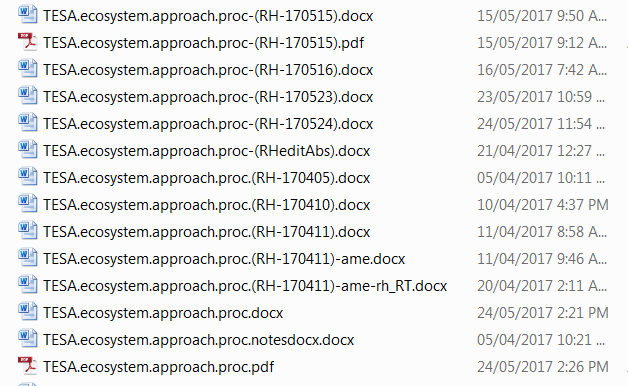
\includegraphics[
        width=\textwidth,
        height=0.8\textheight,
        keepaspectratio]
        {../git-motivation/figures/EAversions.png}
  \end{figure}
}

\frame{\frametitle{So how does Git do all that?}
  \bi
     \item By now you're probably wondering how Git keeps track of everything.
     \item Basically, there is a hidden \lst{.git} folder in each repository.
     \item We'll take a look and explain what we understand.
     \item Look at \lst{refs/} and \lst{objects/}.
     \item So Git keeps track of {\red changes to files}, and so can go back and
        {\red rebuild} any file as per any \lst{commit}. 
     \item Only works for ASCii (text) files, such as \lst{.r}, \lst{.txt},
        \lst{.tex} etc.
     \item This is why you should not commit \lst{.doc}, \lst{.pdf}, 
        \lst{.RData} files (unless you know they will not change).
  \ei
}

\frame{\frametitle{Why you should not commit .RData etc.~files}
  \bi
  \item Collaborator had added \lst{.pdf} and \lst{.RData} files 
     (plus \lst{.r} etc.), but these got updated when the code was run.
  \item Ended up with \lst{.git/objects/pack} being 2.8Gb.
  \item Essentially (I think) Git has to save every version of each file (since
     binary, not just text) -- way more disk space than just the latest version.
  \item I needed space quickly so just deleted four files in 
     \lst{.git/objects/pack}, which freed up 1.6Gb. 
  \item Note that I still have the actual final versions of files (as you would
     if not using Git), but just not the full repository history.
  \item However, when I tried to later do some work and then \lst{commit} I got ...
  \ei
}
 
\frame{\frametitle{Why you should not commit .RData etc.~files}
  \centering
  \begin{figure}
    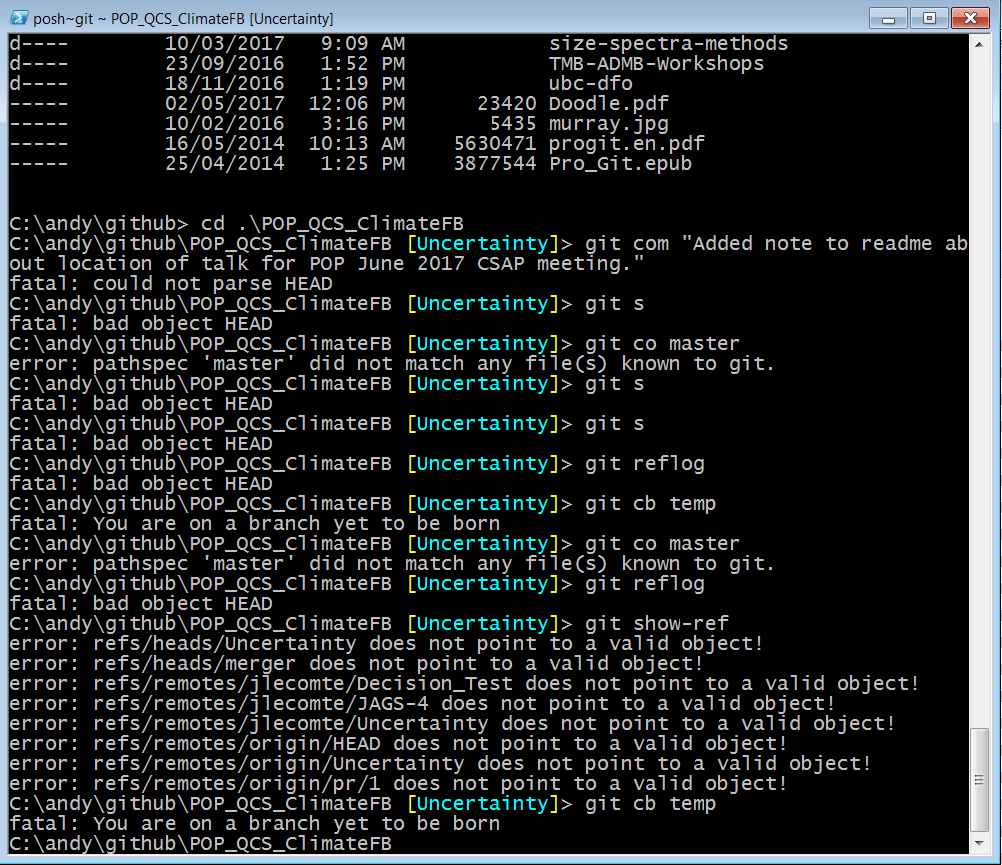
\includegraphics[
        width=\textwidth,
        height=0.8\textheight,
        keepaspectratio]
        {../git-motivation/figures/notGood.png}
  \end{figure}
}



\frame{\frametitle{The \emph{.gitignore} file}
  Each repository can have one \emph{.gitignore} file, in the root directory
  of the repository. This file has names of files or wildcard names such as
  \lstinline{*.dvi} or \lstinline{*.nav} that will be completely ignored by
  \gs. Many compilers make temporary files, the names of which should be added
  to this file to avoid adding these files when adding whole directories
  using commands such as \lstinline{git add r-test}.\\
  \bigskip
  This is important as you will clutter up your repository and have to spend
  time cleaning it all up.\\
  \bigskip
  Anytime you run the command \lstinline{git s} or \lstinline{git s -u} and
  there are files listed that you don't want added to the repository, you
  should add them or a wildcard template encapsulating them to the
  \emph{.gitignore} file so that they are not added inadvertently.
}

\frame{\frametitle{Renaming files}
  \bi
    \item You can rename any files the normal way you do that such as in the
      Windows file explorer.
    \item Once you've renamed your files, check the repository status:\\
      \lstinline{git s}\\
    \item You will see that the files you renamed need to be added again.
      Do this the same way you added them in the first place. You can also
      add a whole directory again and \gs\ is smart enough to only add the
      renamed files.
    \item Check the status again:\\
      \lstinline{git s}\\
      It will show that the file(s) were renamed.
    \item Make a commit:\\
      \lstinline{git com "Renamed files x, y, and z"}\\
    \item Push the commit:\\
      \lstinline{git push}
  \ei
}

\section{Branches}
\frame{\frametitle{Branching overview}
  When you want to add some new code to your project, but don't want to break
  what is already there, you create a new branch. When creating a new branch,
  your starting point is identical to the branch you were in when you created
  the new one.\\
  \bigskip
  Once you have completed your work in the new branch and are satisfied that
  everything is working correctly, you merge the changes into your master
  branch (or any other branch you wish).\\
  \bigskip
  You can also push branches to \gh\ if you feel the branch is going to be a
  longer term project and/or if there are going to be multiple collaborators
  on that new branch.\\
  \bigskip
  It is a good idea to commit all changes before creating a new branch, as
  local changes which haven't been committed will appear in the new branch
  as well.
}

\frame{\frametitle{Creating a new branch}
  \bi
    \item In the \gs, enter your test repository:\\
      \lstinline{cd test}\\
      and see that you are in the \emph{master} branch by looking at the
      prompt.
    \item Create a new branch based off the branch you are currently on:\\
      \lstinline{git cb temp}\\
      You will be automatically placed in the new branch called
      \emph{temp}, and commits you make will now occur in that
      branch only.
    \item To view all local branches:\\
      \lstinline{git branch}\\
      There is an asterisk next to the branch you are currently in.
    \item To switch to another branch, let's say back to \emph{master}:\\
      \lstinline{git co master}\\
  \ei
}

\frame{\frametitle{Make a commit in the new branch}
  \bi
    \item Make sure you are in the new branch:\\
      \lstinline{git co temp}
    \item Create a new file called \lstinline{junk.txt}
    \item \lstinline{git add junk.txt}
    \item \lstinline{git com "Added junk.txt"}
    \item Switch back to \emph{master}:\\
      \lstinline{git co master}
    \item Notice that the file you just added is gone. It only exists in
      the \emph{temp} branch at this point. You will need to merge that
      branch back in to the \emph{master} branch if you want to keep the
      work you did in the other branch.
  \ei
}

\frame{\frametitle{Merging branches}
  \bi
    \item To merge the changes from a branch into another branch:
      \bn
        \item Change to the branch you want to merge into, typically
          \emph{master}:\\
          \lstinline{git co master}
        \item Merge the branch into \emph{master}:\\
          \lstinline{git merge temp}
      \en
    \item Notice that the file you created in the \emph{temp} branch
      now appears in the \emph{master} branch. All commits done in a branch
      which is merged in will be included in the merge step.
    \item Since we are done with that branch for good, we will delete it so
      we don't have unused branches hanging around (next slide).
    \bigskip
    \item If there was a merge conflict, you must fix it at this point. This
      will be covered later in the section about merging remotes, which
      follows the exact same method.
  \ei
}

\frame{\frametitle{Deleting branches}
  \bi
    \item To delete a branch that you are not currently in, in this case
      the \emph{temp} branch:\\
      \lstinline{git branch -d temp}\\
    \item To delete the branch you are currently in, switch to another branch
      first, (e.g. \emph{master}) and then delete the branch:\\
      \lstinline{git co master}\\
      \lstinline{git branch -d temp}\\
    \item If you have unmerged changes in the branch, you will not be allowed
      to delete it. If you want to forcibly delete it, discarding your changes,
      use:\\
      \lstinline{git branch -D temp}\\
      \textbf{Warning - you won't be able to get any of those changes back
        once you do this.}
  \ei
}

\frame{\frametitle{Pushing branches to \gh}
  If you want to push the branch up to \gh, i.e. so others can fetch it and
  edit it, you need to be in the branch locally and:\\

  \lstinline{git --set-upstream origin BRANCH-NAME}\\

  \gs\ is somewhat smart, so if you forget this command and instead type:\\

  \lstinline{git push}\\

  while in the new branch, \gs\ will tell you the command you need.\\
  \bigskip
  Once you've done this for a branch, all you have to do to push future
  commits in this branch is:\\
  \lstinline{git push}\\
  \bigskip
  Check the \gh\ webpage to see that your branch was pushed.
}

\frame{\frametitle{Deleting branches from \gh}
  To remove a branch entirely from \gh:\\
  \lstinline{git push origin --delete BRANCH-NAME}\\
  \bigskip
  The local branch will still exist, so if you want to delete that as well:\\
  \lstinline{git co master}\\
  \lstinline{git branch -d BRANCH-NAME}
}

\section{Network Graph}
\frame{\frametitle{Network Graph}
  The Network Graph is useful when working alone, but especially so when collaborating.\\
  ~\\
  Find it for any repo under \lst{Insights-Graph-Network}.\\
  ~\\
  Look at \url{https://github.com/cgrandin/git-course/network}.\\
  ~\\
  Jump to start, hover over some commits and explain.
}

\frame{\frametitle{From motivation talk}
  Screenshot from 30th May shows (and next page):
  ~\\
  ~\\
  \includegraphics[
     width=\textwidth,
     height=0.6\textheight,
     keepaspectratio]
     {../git-motivation/figures/netWorkGraph1}
}

\frame{\frametitle{From motivation talk}

  \includegraphics[
     width=\textwidth,
     height=0.6\textheight,
     keepaspectratio]
     {../git-motivation/figures/netWorkGraph2}

  Andy had done nothing for a while.

}

\frame{\frametitle{From motivation talk}
  \includegraphics[
     width=\textwidth,
     height=0.6\textheight,
     keepaspectratio]
     {../git-motivation/figures/netWorkGraph1}\\
  The graph was for {\red Andy's repo}, so Andy is at the top.\\
  Chris's name shows up because he had pushed commits that Andy did not 
    yet have.\\
  So the graph shows that Andy should get caught up before continuing on 
    this project.\\
  This took three commands, resulting in:
  \includegraphics[
     width=\textwidth,
     height=0.6\textheight,
     keepaspectratio]
     {../git-motivation/figures/netWorkGraph3}
}



\frame{\frametitle{From motivation talk}
  \includegraphics[
     width=\textwidth,
     height=0.6\textheight,
     keepaspectratio]
     {../git-motivation/figures/netWorkGraph3}
  ~\\
  All files that Chris edited got updated, plus Andy then had any new files
    that Chris created, and our folder structures are identical.\\
  ~\\
  Chris's name doesn't show up, even though he did a lot of the work.\\
  ~\\
  It is ``{\red about code not ego}''.
}
  
\frame{\frametitle{Network Graph}
  \bi
    
    \item Live version: \url{https://github.com/andrew-edwards/git-course/network}\\
    \item What about: \url{https://github.com/cgrandin/git-course/network}\\
    \item Andy's name (probably) doesn't show up.\\
    \item But we both did work -- can see who did what by hovering 
      over commits.\\
    \item It is ``{\red about code not ego}''.
  \ei
}

\frame{\frametitle{Understanding the Network Graph}

  Now, for hake assessment:
    \url{https://github.com/andrew-edwards/hake-assessment/network}\\

  Click on \lst{cgrandin} on that graph, to see the graph of Chris's repo.\\
  Andy does not show up on that because he has not committed anything new (Chris
    has everything Andy has done).




  Paraphrasing from (slightly dated) \url{https://github.com/blog/39-say-hello-to-the-network-graph-visualizer}\\
  


}

\section{Remotes}
\frame{\frametitle{Remotes overview}
  Once you have created a repository on \gh\ and uploaded some files, you may
  want to start collaboration with others. To do this, send them the URL of
  your \gh\ repository, and ask them to \emph{Fork} it on \gh. Once they have
  done that and cloned your repository, everyone involved will need to add
  each other's repository as a \emph{remote} so that all changes can be merged.\\
  \bigskip
  Adding remotes has to be done once for each project. Once you have added
  someone, their remote information remains on your local computer. \gh\ has
  some smart programming, which detects merges between remotes and will keep
  track of the project and all its contributions.\\
  \bigskip
  The network graph is a great place to look at what has happened on a given
  repository.
}

\frame{\frametitle{Adding remotes}
  \bi
    \item Once everyone has \emph{Forked} on \gh, you must add each person as
      a \emph{remote}. They must also add everyone else as remotes. Everyone
      must trade URLs, and add each other person like this:\\
      \lstinline{git remote add REMOTE-NAME REMOTE-URL}\\
      where:\\
      \bi
        \item \lstinline{REMOTE-NAME} is a name you make up that you will
          remember. I use first initial followed by last name for everyone,
          so they have the same syntax. e.g.: cgrandin, aedwards, rforrest.
        \item \lstinline{REMOTE-URL} is the URL on \gh\ where the person's
          repository can be found. e.g.:\\
          \url{https://github.com/cgrandin/git-course}.
      \ei
    \item To view all remotes you have set up:\\
      \lstinline{git r}
  \ei
}

\section{Fetching and merging remotes}
\frame{\frametitle{Fetching overview}
  Once you have set up your remotes, you can fetch other people's commits.
  Before continuing work on your project, you should always check \gh, and
  see if your collaborators have been working, and if so, what their commits
  were. At this stage you get a general idea of what has been done since
  you last looked at the repository. Once you have familiarized yourself with
  the changes in a broad sense, you will want to merge them into yours.\\
  \bigskip
  Find the most recent commit on \gh's \emph{Network Graph}. It will have
  one person's name associated with it. That is the person you will fetch
  and merge in.\\
  \bigskip
  There may be some disarray in the network graph, but you can just merge
  each person's repository into yours in succession if you wish, which
  will clean up the network graph.
}

\frame{\frametitle{Fetching other people's changes}
  To fetch someone's changes:\\
  \bigskip
  \lstinline{git fetch REMOTE-NAME}\\
  \bigskip
  where \lstinline{REMOTE-NAME} is one in the list of remotes you have set up.
  This command fetches everything in the person's repository, including
  all branches. Running this command does not affect your repository
  in any way. The fetch stores the information in a cache, awaiting
  your command to merge.
}

\frame{\frametitle{Comparing the fetched repository with yours}
  Once you've fetched someone's repository, you can exactly see what has
  changed compared to yours. This is called \emph{Diff-ing}.
  \bi
    \item To compare the changes in their master to yours (make sure you are in
      the master branch in \gs):
      \lstinline{git diff REMOTE-NAME/master}\\
      or using the \emph{Difftool} if you have it set up:\\
      \lstinline{git difftool REMOTE-NAME/master}
    \item This will show you exactly what changes to each file you are about
      to merge into your repository.
    \item In general, I use \emph{diff} if there are only minor changes
      and \emph{difftool} if there are more changes or if more than one file
      has been changed.
  \ei
}

\frame{\frametitle{Merging the fetched repository into yours}
  To merge the fetched repository's master branch into yours:\\
  \lstinline{git merge REMOTE-NAME/master}\\
  note that the merge will happen in the branch you are currently in, so make
  sure you are in the \lstinline{master} branch.\\

  \bigskip

  At this point, you will either be up-to-date, meaning there were no merge
  conflicts, or you will have one or more merge conflicts. If you are
  up-to-date, you need to push back to your repository to complete the merge
  step:\\
  \lstinline{git push}\\
  If you have conflicts, you need to fix them before continuing work.
}

\frame{\frametitle{Exercise on remotes and merging - 1}
  \bn
    \item Each group of four sitting together will collaborate. Each person
      in the group gets a number: 1, 2, 3, or 4.
    \item Person 1 will set up a new repository on \gh\ called
      \lstinline{help-friends}
    \item Person 1 copies \lstinline{git-course/exercise-files/helpFriends.txt}
      into their new repository (on their computer).
    \item \lstinline{add}, \lstinline{commit}, \lstinline{push}.
      Check Network Graph.
    \item Persons 2, 3 and 4 then fork and clone the repository.
    \item All team members must add everyone else as a remote:\\
      \lstinline{git remote add REMOTE-NAME REMOTE-URL}\\
      (run once for each team member other than yourself), e.g.:\\
      \lstinline{git remote add aedwards https://github.com/andrew-edwards/help-friends}
    \item Run the command \lstinline{git r} to see your list of remotes. Make
      sure everyone in your group is on the list.
    \item Everyone does a few edits on their paragraph
      (see \lstinline{helpFriends.txt}).
    \item \lstinline{commit} a few times, \lstinline{push}.
      Check Network Graph.
  \en
}

\frame{\frametitle{Exercise on remotes and merging - 2}
  \bn
    \item Explore Network Graph (hover over the commits).
    \item Whoever is furthest behind (not that it matters), \lstinline{fetch}
      and \lstinline{merge} from the person who's furthest ahead:
      \bi
        \item \lstinline{git fetch REMOTE-NAME}
        \item \lstinline{git diff REMOTE-NAME/master}
        \item \lstinline{git merge REMOTE-NAME/master}
        \item \lstinline{git push}
        \item Check Network Graph (have to refresh).
        \item Check your collaborator's Network Graph (helpful if you care whether
          they have caught up with you).
      \ei
    \item Repeat step 2 until everyone is caught up.
    \item Step 2 is essentially all you have to (ever) do to keep collaborating on this repo.
  \en
  Note that \gs\ auto-completes with \lstinline{<TAB>}, e.g. \lstinline{git merge <TAB>}
}

\frame{\frametitle{Exercise on remotes and merging - 3}
  \bn
    \item Note that if person A has fetched and merged B's work, person C
      can just fetch and merge from A (not from A and B -- A has already done that).
    \item On your repo website, go to Code and navigate to and click on \emph{helpFriends.txt}.
    \item See what Raw, Blame and History buttons do.
    \item Your Network Graph acts as a to-do list. Each person you have not merged
      with will be below you on the graph in a new slot. If there are no names below yours,
      you have no unmerged commits and are up-to-date.
  \en
}



\frame{\frametitle{Deleting or renaming remotes (may occasionally need)}
  \bi
    \item To delete someone as a remote:\\
      \lstinline{git remote delete REMOTE-NAME}\\
      where \lstinline{REMOTE-NAME} is the name you made up when you added them.
    \item To rename a remote:\\
      \lstinline{git remote rename OLD-NAME NEW-NAME}\\
      where \lstinline{OLD-NAME} is the name you made up when you added them and
      \lstinline{NEW-NAME} is the name you want to change it to.
    \item To see your changes, use:\\
      \lstinline{git r}
  \ei
}

\begingroup
\small
\frame{\frametitle{Conflicts - what if two people have edited the same lines?}
  The merge message will tell you which files are conflicting. Open those
  files one by one, and you will see the conflicted section bracketed like the
  following:\\
  \bigskip
  \lstinline{<<<<<<< HEAD}\\
  Line(s) of text/code which are currently in your file.\\
  \lstinline{=======}\\
  Line(s) of text/code which are trying to merge in, but conflict.\\
  \lstinline{>>>>>>> BRANCH-NAME}\\
  \bigskip
  where \lstinline{BRANCH-NAME} is the name of the branch you are trying to
  merge in from the previously-issued command:\\
  \lstinline{git merge BRANCH-NAME}\\
  All you do is remove the bracketing lines (\lst{<<<...} and \lst{>>>...}), 
  the \lstinline{=======} line,
  and choose one of the line(s) of text/code to keep, or edit the line(s)
  to be something else entirely. Once you are done fixing each conflicted file,
  you need to commit the merge conflict and push the result:\\
  e.g.~\lstinline{git com "Kept Dave's edits as more consistent with 
  remaining text."}\\
  \lstinline{git push}
}
\endgroup

\frame{\frametitle{Dealing with merge conflicts - mergetool}
  You can also use a mergetool such as DiffMerge to fix the conflicts. It is
  easier in that it will open a new session for each conflict and place you
  at the correct place. You won't have to see the bracketing markers and the
  files will be edited by the mergetool to what you want. If you want to try
  the mergetool, after a merge conflict message, run:\\
  \lstinline{git mergetool}\\
  \bi
    \item The left panel is what is in the branch you are in when you called
      the merge command.
    \item The middle panel is what you will end up with once finished.
    \item The right panel is what is in the branch you are trying to merge
      in.
  \ei
  Once finished, click the X to close and the next conflicted file will pop
  up in a new session of DiffMerge. Once all conflicts have been resolved,
  issue a commit and push to complete to merge:\\
  \lstinline{git com "Merge conflict resolved."}\\
  \lstinline{git push}
}

\frame{\frametitle{\gh\ - Add collaborators}
  If your \gh\ repository is public, anyone can post an issue. If you want
  someone to be able to:
  \bi
    \item Set assignees to issues
    \item Receive notifications when you reply to their issue
  \ei
  You need to add them as a collaborator. Select the \emph{Settings} tab and
  then the \emph{Collaborators} button. Type their \gh\ username in and send
  them an invitation to collaborate.
}

\section{Stashing}
\frame{\frametitle{Stashing overview}
  If you are in the middle of working on something, but you need to change
  branches for some reason, you can \emph{stash} your changes and apply
  them back later. Let's say you are working in the master branch. To
  stash all changes in master:\\
  \lstinline{git stash}\\
  then change branches, and do whatever you like. To get those changes back,
  switch back to master:\\
  \lstinline{git co master}\\
  and apply the stashed changes:\\
  \lstinline{git stash pop}\\
  Note that nothing is committed, this just lets you put on hold your work
  in progress and come back to where you left off.
}

\frame{\frametitle{Stashing - make it into a branch}
  If you leave a stash for awhile and have made commits since the stash,
  then try to reapply it, you may get conflicts. The best way to apply a stash
  if you have modified things since you stashed is to let git create a branch
  for the stash, which you can then look at and edit if you wish before merging
  back into your master or other working branch:\\
  \bigskip
  \lstinline{git stash branch BRANCH-NAME}\\
  \bigskip
  where \lstinline{BRANCH-NAME} is the name you want to call the new branch.
  You can then merge this branch in as outlined in the merging slides and
  resolve conflicts in the same way as with remotes or other local branches.
}

\section{Undoing things}
\frame{\frametitle{Changing the commit message in the last commit}
  If you make a commit, then realize that your message had a spelling error,
  or needed more information in it, you can change the commit message:\\
  \bigskip
  \lstinline{git commit --amend -m "Correct message."}\\
  \bigskip
  This only works on the last commit. You can't change any other commit message
  using \emph{amend}.\\
  If you already pushed the commit before realizing that the message needs
  modification, do this:\\
  \bigskip
  \lstinline{git push --force}\\
  \bigskip
  after making the amendment to the commit message. You can also add more files
  before issuing the amendment commit and those files will be added to the commit
  you are amending. You can't add changes to file content this way though, you'll
  need to do another commit for that.
}

\frame{\frametitle{Undoing a commit}
  If you make a commit followed by other commits, then realize you want to undo
  the earlier commit, you use \emph{revert}:\\
  \bigskip
  \lstinline{git revert HASH}\\
  \bigskip
  where \lstinline{HASH} is the hash for the commit you want to undo (20-byte string)
  Remember that \gs\ is smart enough that you only need the first five digits:\\
  \bigskip
  \lstinline{git revert 1ef1d}\\
  \bigskip
  It is important to make a lot of commits, each with only small changes.
  You can only revert the whole commit, not parts.
}

\frame{\frametitle{Undoing changes not yet committed}
  If you've made a mess in your working directory and you want to change
  everything back to the way it was on the last commit:\\
  \bigskip
  \lstinline{git reset --hard HEAD}\\
  \bigskip
  If you've messed up a single file and just want that one file to go back
  to the way it was on the last commit:\\
  \bigskip
  \lstinline{git checkout HEAD file/to/restore.r}\\
  \bigskip
  Warning - running these commands will delete the changes you have made.
  Since you have not committed any changes, they will be lost. Make sure
  you are certain you don't need the changes before running these commands.
  If you aren't sure if you need the changes again in the future, use
  \lstinline{git stash} instead.
}

%% Git tower webpage:
%% https://www.git-tower.com/learn/git/ebook/en/command-line

\end{document}
